\documentclass{classrep}
\usepackage[utf8]{inputenc}
\frenchspacing

\usepackage{graphicx}
\usepackage{rotating}
\usepackage[usenames,dvipsnames]{color}
\usepackage[hidelinks]{hyperref}
\usepackage{float}
\usepackage[table,xcdraw]{xcolor}

\usepackage{amsmath, amssymb, mathtools}

\usepackage{fancyhdr, lastpage}
\pagestyle{fancyplain}
\fancyhf{}
\renewcommand{\headrulewidth}{0pt}
\cfoot{\thepage\ / \pageref*{LastPage}}

\renewcommand{\refname}{Bibliografia}

% bullet itemize
\renewcommand{\labelitemi}{\textbullet}

\studycycle{Informatyka stosowana, studia dzienne, II st.}
\coursesemester{2}

\coursename{Zastosowanie informatyki w medycynie}
\courseyear{2020/2021}

\courseteacher{dr hab. inż. Agnieszka Wosiak}
\coursegroup{środa, 13:30} %wpisałem start wykładu bo raz wykład raz laby

\author{%
\\
  \studentinfo[234053@edu.p.lodz.pl]{Paweł Galewicz}{234053}\\
  \studentinfo[234067@edu.p.lodz.pl]{Bartosz Jurczewski}{234067}\\
  \studentinfo[234102@edu.p.lodz.pl]{Zbigniew Nowacki}{234102}\\
  \studentinfo[234128@edu.p.lodz.pl]{Piotr Wardęcki}{234128}
}

\title{Zadanie 1: Czy warto się szczepić?}

\begin{document}
\maketitle
\thispagestyle{fancyplain}
\clearpage

%%%%%%%%%%%%%%%%%%%%%%%%%%%%%%%%%%%%%%%%%%%%  Cel
\section{Cel}
    Przygotowanie sprawozdania, które może posłużyć w zwiększaniu świadomości wśród rodziny, przyjaciół czy znajomych o pozytywnym wpływie szczepionek na zdrowie publiczne.

%%%%%%%%%%%%%%%%%%%%%%%%%%%%%%%%%%%%%%%%%%%%  WPROWADZENIE
% \section{Wprowadzenie}

%%%%%%%%%%%%%%%%%%%%%%%%%%%%%%%%%%%%%%%%%%%%  OPIS IMPLEMENTACJI
\section{Opis implementacji}
    Algorytmy oraz przygotowane do nich testy zostały zaimplementowane za pomocą języka Python w wersji 3.8.2.
    Wykorzystano w nim biblioteki \textit{NumPy}, \textit{Sklearn}, \textit{Pandas} i \textit{Seaborn}.

%%%%%%%%%%%%%%%%%%%%%%%%%%%%%%%%%%%%%%%%%%%%  Badania
\section{Badania}
    Dane użyte do badań pochodzą ze Stanów Zjednoczonych Ameryki z okresu 1928 do 2011. Zawierają cotygodniowe ilości zakażonych i są podzielone na stany. Do samych badań pominęliśmy Alaskę oraz Hawaje ponieważ dołączyły się do stanów w późnych latach 50 XX wieku.

\subsection{Odra}
    Dla stanu Kalifornia przygotowaliśmy wykres zakażeń na odrę zależnie od czasu. Zieloną linią wyznaczyliśmy rok wprowadzenia szczepionek - rok 1963.

    \begin{figure}[H]
        \centering
        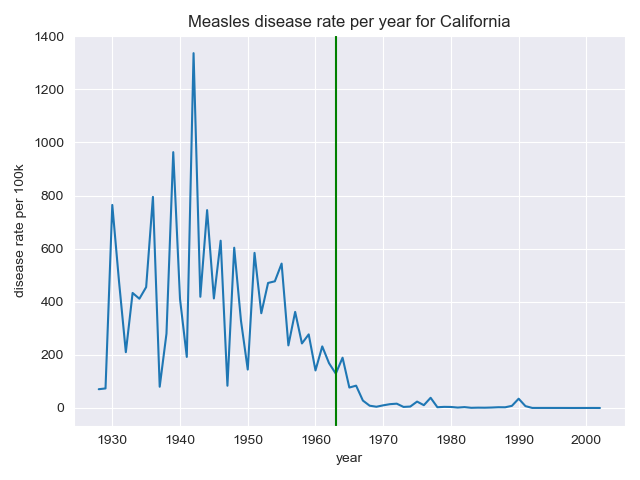
\includegraphics[width=0.9\textwidth]{images/images1/Figure_1.png}
        \caption{Wskaźnik zachorowań na odrę rocznie w Kalifornii.}
        \label{fig1}
    \end{figure}

\subsection{Histogramy}
    Dla dekad 1950, 1960 oraz 1970 przygotowaliśmy oddzielne histogramy z oraz bez transformacji pierwiastkowej.
    Rysunek 2 prezentuje nasze wyniki.

    \begin{sidewaysfigure}[!ht]
        \centering
        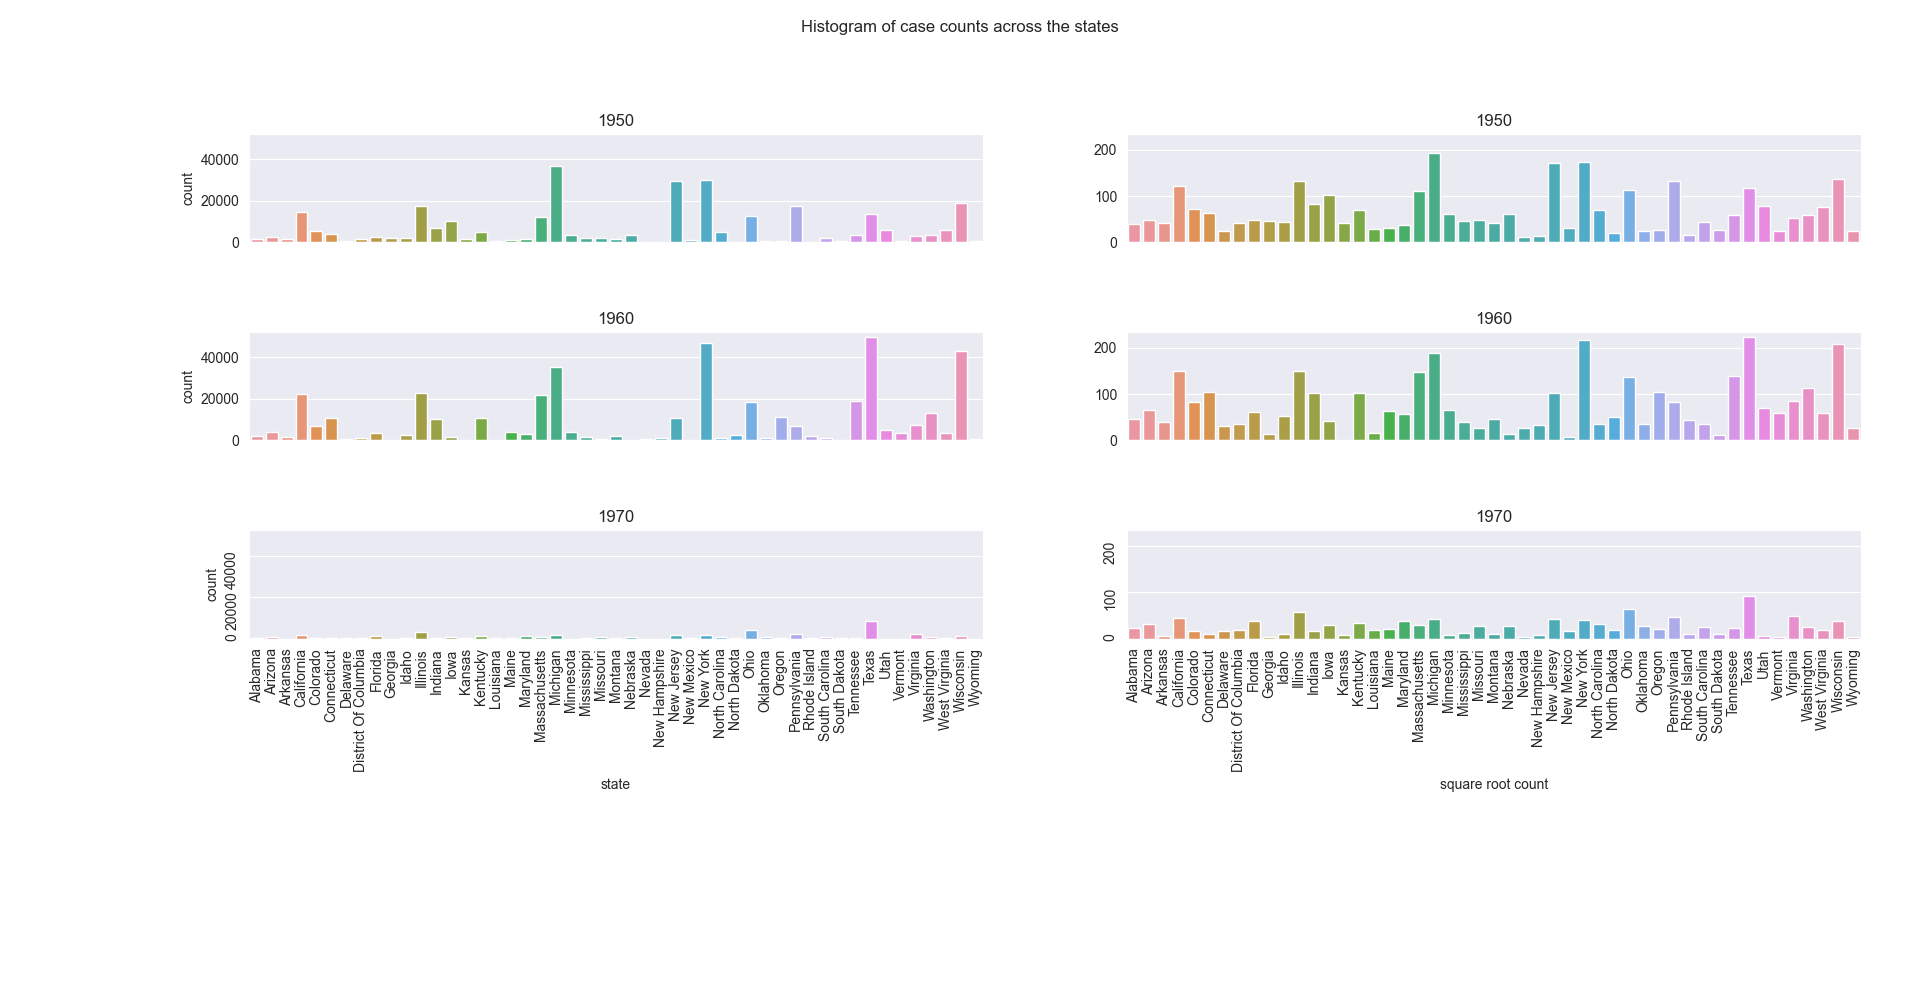
\includegraphics[width=1\textwidth]{images/images1/Figure_2.png}
        \caption{Histogram przypadków obejmujący wszystkie stany.}
        \label{fig2}
    \end{sidewaysfigure}

\subsection{Odra w każdym ze stanów}
    Szczepionka na odrę została wynalezione w 1963. Już kilka lat później w Kalifornii nastąpił znaczący spadek zachorowań i prawie zrównał się z zerem.
    % Napisać wiecej jak dodamy nowy wykres! Oraz podmienic tresc
    % linia dla Kaliforni
    % Jak wyglądało w innych stanach? Czy zmalało?

    \begin{figure}[H]
        \centering
        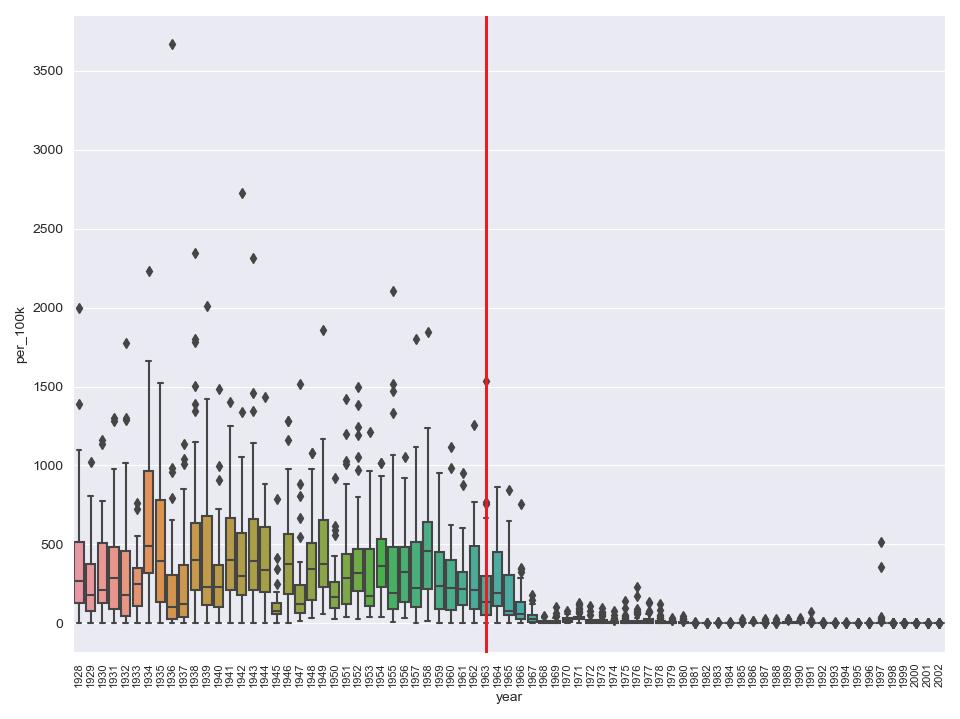
\includegraphics[width=1\textwidth]{images/images1/Figure_33.png}
        \caption{Świecowa reprezentacja liczby zachorowań dla stanu Kalifornia.}
        \label{fig3a}
    \end{figure}

    Wykres przedstawiający liczbę zakażeń dla każdego stanu, klarownie pokazuję rok szczepienia na 1963.

    \begin{figure}[H]
        \centering
        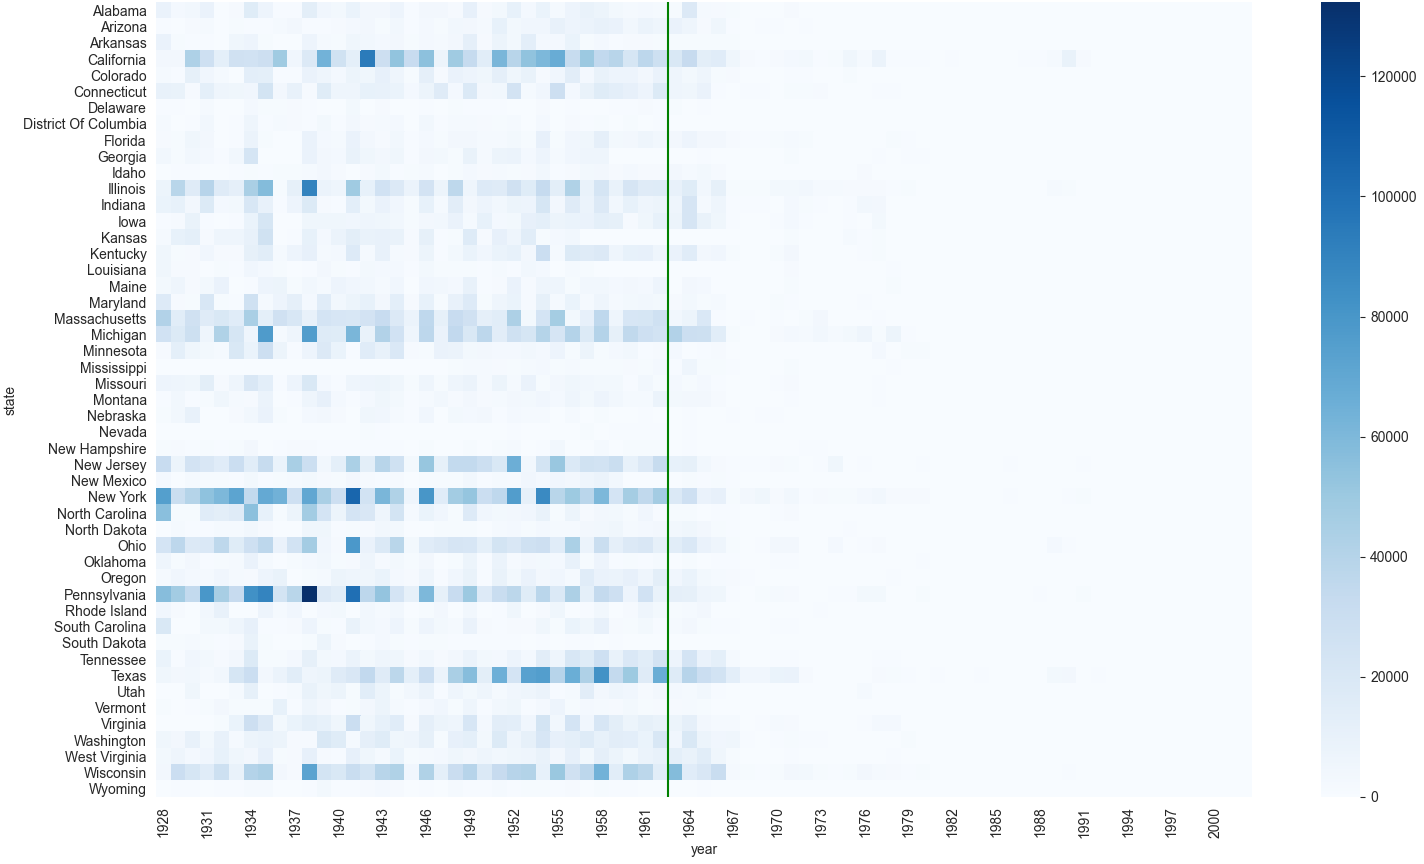
\includegraphics[width=1\textwidth]{images/images1/Figure_7.png}
        \caption{Heatmapa dla każdego ze stanów, liczba zachorowań na przestrzeni lat.}
        \label{fig3b}
    \end{figure}

\subsection{Wpływ szczepionek na zachorowania}
    Szczepionka na Polio masowa zaczęła być używana w 1955 roku.
    \begin{figure}[H]
        \centering
        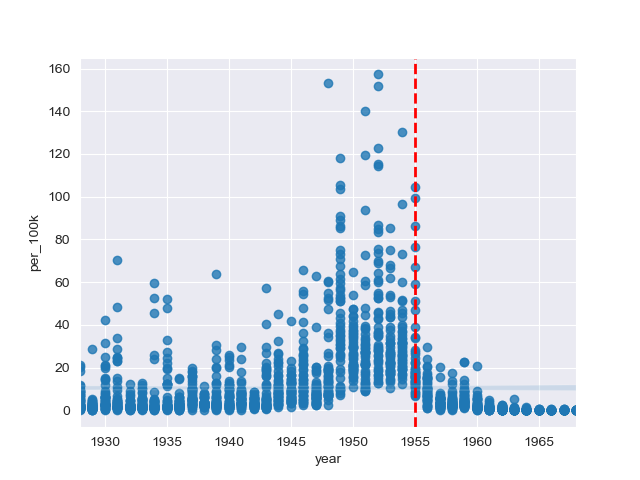
\includegraphics[width=1\textwidth]{images/images1/Figure_4.png}
        \caption{Wskaźnik zachorowań na polio rocznie w USA.}
        \label{fig4}
    \end{figure}

    Szczepionka na odrę została wprowadzona w 1968 roku, a wynaleziona w 1963 roku.
    \begin{figure}[H]
        \centering
        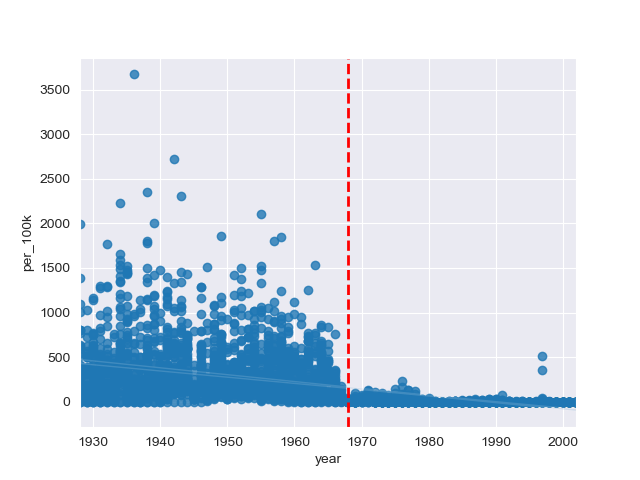
\includegraphics[width=1\textwidth]{images/images1/Figure_5.png}
        \caption{Wskaźnik zachorowań na odrę rocznie w USA.}
        \label{fig5}
    \end{figure}

    Szczepionka na wirusa zapalenia wątroby typu A została wprowadzona w USA w roku 1995. W europie było to w 1991 roku.
    \begin{figure}[H]
        \centering
        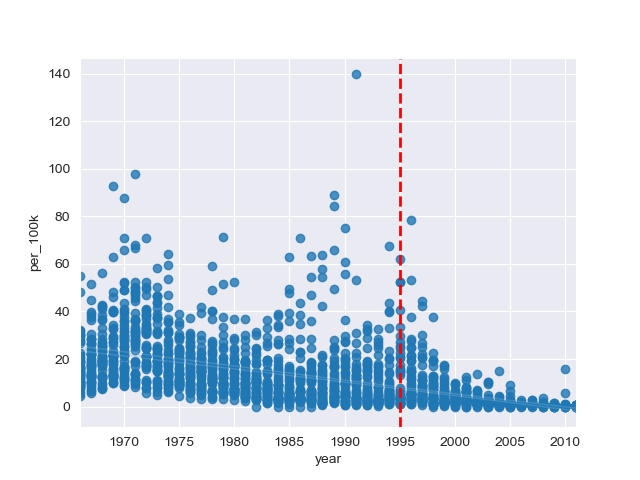
\includegraphics[width=1\textwidth]{images/images1/Figure_6.png}
        \caption{Wskaźnik zachorowań na wirusa zapalenia wątroby typu A rocznie w USA.}
        \label{fig6}
    \end{figure}

%%%%%%%%%%%%%%%%%%%%%%%%%%%%%%%%%%%%%%%%%%%% Wnioski
\section{Wnioski}

    \begin{itemize}
        \item Szczepienia realnie wpływają na liczbę zachorowań.
        \item Trend antyszczepionkowców nie ma żadnych przesłanek naukowych. Prosta analiza danych historycznych potwierdziła tezę o stosowności szczepionek.
    \end{itemize}

% \newpage

\nocite{*}
% \begin{thebibliography}{0}
    
    % \bibitem{docker}
    % \textsl{Jupyter Notebook Python, Spark Stack}
    % \url{https://hub.docker.com/r/jupyter/pyspark-notebook}
    
% \end{thebibliography}
\end{document}
